\documentclass[11pt]{article}
\usepackage[margin=1in]{geometry}
\usepackage{fontspec,amsmath,booktabs,threeparttable,graphicx,placeins,natbib,xurl,setspace,adjustbox}
\setstretch{1.15}
\graphicspath{{../figs/}}
\newcommand{\rtincoded}{104}
\newcommand{\rtinfull}{15}
\newcommand{\rtininformed}{54}
\newcommand{\rtiagreeinfo}{92}
\newcommand{\rtiagreedisp}{74}
\newcommand{\rtiasof}{29 October 2026}
\newcommand{\rtindrawn}{1,665}
\newcommand{\rtinfiled}{996}
\newcommand{\rtinpastthirty}{455}
\newcommand{\rtianyextg}{28.7}
\newcommand{\rtiinfoextg}{14.2}
\newcommand{\rtianytn}{12.9}
\newcommand{\rtianytnw}{7.0}
\newcommand{\rtianyka}{52.6}
\newcommand{\rtianytg}{1.1}
\newcommand{\rtibtn}{1.1}
\newcommand{\rtisetn}{5.8}
\newcommand{\rtimdetn}{16.2}
\newcommand{\rtibother}{3.6}
\newcommand{\rtiseother}{3.9}
\newcommand{\rtimdeother}{10.9}
\newcommand{\rtibextg}{10.9}
\newcommand{\rtiseextg}{9.3}
\newcommand{\rtimdeextg}{26.1}

\usepackage[font=small,labelfont=bf]{caption}
\usepackage[hidelinks]{hyperref}
\setlength{\emergencystretch}{2em}
\title{Measuring the Right to Know:\\Early Evidence from an Online RTI Audit in India}
\author{Priyadarshi Amar \and Gaurav Sood}
\date{Working draft: data through \rtiasof{}}
\begin{document}
\maketitle
\begin{abstract}
How often does an online Right to Information (RTI) application produce the information requested? We study applications for public authorities' own RTI records in Tamil Nadu, Telangana, Karnataka, Delhi, and Maharashtra. By \rtiasof{}, \rtinfiled{} of \rtindrawn{} planned applications had been filed, and \rtinpastthirty{} had at least thirty days of follow-up. Among these applications outside Telangana, \rtianyextg{} percent had a recorded response within thirty days and \rtiinfoextg{} percent had supplied at least some requested information. Missing portal and postal replies mean that these figures understate responses not captured in the study records. We also randomly vary whether requests mention statutory deadlines and penalties. The estimated effects are imprecise. These interim findings document a gap between administrative responses and information provision among the offices studied; they do not establish a national compliance rate.
\end{abstract}

\section{Introduction}
An information request can receive a response without receiving an answer. An office may transfer the application, ask for a fee, or mark the case disposed without supplying the requested records. Assessing access to information therefore requires evidence on what applicants receive, as well as whether officials respond.

We examine this distinction in an audit of India's Right to Information system. Public authorities in Tamil Nadu, Telangana, Karnataka, Delhi, and Maharashtra received a common request for records of their handling of RTI applications. Among applications with at least thirty days of follow-up outside Telangana, \rtianyextg{} percent had a recorded response within thirty days, while \rtiinfoextg{} percent had supplied at least some requested information. These figures describe the records available during an ongoing study. Some replies remain uncollected, particularly in Telangana, and the offices filed first differ from the full sample.

India's RTI system has an extensive record of empirical assessment. National assessments led by the Right to Information Assessment and Analysis Group (RaaG) examined applicants' experiences, filed requests, inspected public authorities, and compared reported performance with information obtained in practice \citep{raag2009,raag2014}. Research on implementation and information commissions documents the organizational and enforcement problems that shape access \citep{relly2020,sns2025}. Our study builds on this work by sending a common request across offices listed on online portals and linking each application to dated responses and the contents of available reply documents.

The audit also tests whether explicitly mentioning statutory deadlines and penalties changes an office's response. International experiments show that request wording can matter, but the effect depends on the information sought and the institutional setting \citep{worthy2017,grimmelikhuijsen2019,spac2018,spac2025}. Both versions of our request use the RTI process; only one includes the additional legal reminder. The estimates reported here are too imprecise to determine whether that reminder improves responsiveness.

\section{Related research}
\subsection{Access to information in India}
The Indian literature examines both the benefits of using RTI and the obstacles to obtaining information. \citet{peisakhin2010} and \citet{peisakhin2012} provide experimental evidence that RTI can help citizens obtain public services in Delhi. Those studies ask whether invoking information rights changes access to a service. We ask whether an application produces the records requested, an earlier step in many uses of the law.

The closest precedents for our descriptive approach are the RaaG assessments. The first assessment combined interviews, inspections, analysis of applications, and requests filed by the research team \citep{raag2009}. The later assessment compared information reported by public authorities with the results of applications filed by researchers and with applicants' accounts \citep{raag2014}. It also recognized that the content of a request and the authorities selected affect measured success. Our common request follows this approach: asking each office about its own RTI records reduces variation in subject matter, though differences in record-keeping can still make the same request more demanding in one office than another.

Studies of implementation help explain why a common legal entitlement may produce different experiences. Drawing on interviews and information-commission decisions, \citet{relly2020} identify political will, bureaucratic culture, civic engagement, and administrative capacity as influences on RTI implementation. The information-commission report by \citet{sns2025} documents vacancies, backlogs, and limited use of penalties during its reporting period. These studies concern institutions that support and enforce disclosure. Our observations concern the initial response to an application; they do not measure the eventual resolution of an appeal.

\subsection{Request wording, identity, and administrative burden}
Field experiments provide evidence that invoking information law can improve responsiveness. \citet{worthy2017} compare formal FOI requests with informal requests in England; \citet{grimmelikhuijsen2019} replicate that contrast in the Netherlands. \citet{spac2018} find that a legal reference increases responses from Slovak municipalities, whereas a moral appeal does not. These comparisons motivate our experiment but differ from it: our control request is already a formal RTI application. The treatment tests the additional value of mentioning deadlines and penalties within that process.

Wording can change several aspects of a response. \citet{cuillier2010} find that threatening letters produce faster responses and lower fees, while friendly letters elicit more helpful behavior. \citet{benaaron2017} show that information about peer compliance affects the timing and completeness of responses by local governments. More recently, \citet{spac2025} find that requests for more data receive fewer responses, and that a legal reference moderates this effect. Together, these findings suggest that a reminder's effect may depend on both the work required to answer and the incentives officials perceive. Our experiment does not separately identify these mechanisms.

Requester identity can also affect access. \citet{michener2020} find different responses to institutional and noninstitutional requesters in Brazil, even when identifying cues in the requests are limited. In Uruguay, \citet{pineiro2018} find that the benefit of invoking the law differs by requester gender. \citet{cicatiello2024} document regional differences in the treatment of prominent requesters in Italy. These findings make it important to distinguish request wording from applicant characteristics. We randomize the legal reminder but do not manipulate identity, and comparisons between our filers cannot isolate an identity effect.

\subsection{What counts as successful access?}
Response frequency, speed, and quality need not improve together. Repeated audits in Mexico find more frequent answers and more information over time, alongside longer delays and no improvement in response quality \citep{lagunes2019}. This motivates our separate measures of office action, replies, and information supplied. A transfer or fee demand may be a step toward disclosure, but it does not establish that the applicant received the requested records.

The information sought also matters. \citet{berliner2018} show that citizens' requests in Mexico cover diverse public and private concerns. A standardized request offers greater comparability across offices at the cost of narrower coverage of that demand. Our results therefore concern access to an authority's own RTI records, rather than the full range of questions citizens put to government.

\section{Study design}
\subsection{Requests and office selection}
Each application asks for the authority's RTI records for the preceding twelve months and its annual summary of RTI activity, reported under Section 25. The authority may provide records for individual applications, counts by category, or totals for the period. The request does not seek applicants' names or addresses. Allowing several reporting formats accommodates differences in how offices maintain their records.

We select offices from the lists of public authorities on state RTI portals. In Tamil Nadu, the sample uses quotas within each department for department headquarters, head-of-department offices, and subordinate offices. In the other states, offices are sampled within department groups, subject to caps. Table~\ref{tab:tab_sample} reports the number selected, the number filed, and the number with at least thirty days of follow-up.

Filing is incomplete at the date of this analysis, and filing order was not randomized. The offices with thirty days of follow-up are consequently a subset of the selected offices. The state-level results describe that subset, rather than all offices on a state's portal. Combining the states does not yield a nationally representative sample.
\begin{table}[!htbp]
\centering
\caption{Sample and filing by state}
\label{tab:tab_sample}
\small
\begin{adjustbox}{max width=\textwidth}
\begin{threeparttable}
\begin{tabular}{lrrrrrrl}
\toprule
State & Frame & Drawn & Plain / legal & Filed & Filed (\%) & Past day 30 & Filing window \\
\midrule
Tamil Nadu & 17,417 & 1,000 & 700 / 300 & 525 & 52.5 & 140 & 26 Aug to 28 Oct \\
Telangana & 3,401 & 375 & 262 / 113 & 218 & 58.1 & 187 & 04 Sep to 24 Oct \\
Karnataka & 1,800 & 180 & 126 / 54 & 148 & 82.2 & 78 & 11 Sep to 28 Oct \\
Delhi & 223 & 44 & 30 / 14 & 44 & 100.0 & 22 & 19 Sep to 26 Oct \\
Maharashtra & 328 & 66 & 46 / 20 & 61 & 92.4 & 28 & 15 Sep to 27 Oct \\
\midrule
All & 23,169 & 1,665 & 1,164 / 501 & 996 & 59.8 & 455 & 26 Aug to 28 Oct \\
\bottomrule
\end{tabular}
\begin{tablenotes}[flushleft]\footnotesize
\item \textit{Notes:} Data as of 29 October 2026. Past day 30: filed by 29 September, so the 30-day limit in s.7(1) has passed. Tamil Nadu is drawn by department $\times$ tier quotas, other states proportionally to department group with a cap.
\end{tablenotes}
\end{threeparttable}
\end{adjustbox}
\end{table}

\FloatBarrier

\subsection{The legal reminder}
The treatment letter includes a paragraph referring to the Section 7(1) deadline and Section 20 penalties. The control letter omits that paragraph. Maharashtra's portal requires a shorter request, so we also report estimates excluding Maharashtra.

Treatment is assigned within department and office level in Tamil Nadu. In Telangana and Karnataka, it is assigned within the filing batch. In Delhi and Maharashtra, it is assigned within state and batch. The regressions account for these assignment groups. Additional department-group controls in some specifications adjust for office composition; they are not part of the assignment procedure in those states.

Applicants use their own identities. Some research-assistant identifiers refer to the same person, and phone availability differs between filers. Differences between filers therefore combine identity, address, and phone access. We do not interpret them as causal effects of any one characteristic.

\section{Data and outcomes}
The analysis combines application assignments, filing records, office emails, and reply documents available through \rtiasof{}. We count an application as filed when it has a registration number or a portal acknowledgment. Repeat submissions are linked to the original sampled office. There are \rtinfiled{} filed applications out of \rtindrawn{} planned, of which \rtinpastthirty{} have at least thirty days of follow-up.

We measure outcomes within thirty days of filing. The filing date comes from the portal where available and otherwise from the filing record. For reply documents, we use the letter's date when legible and otherwise its recorded arrival date. Measured response times therefore do not consistently represent the date on which information reached the applicant. The common thirty-day window provides a comparable outcome; it is not a determination of the legal deadline in each case.

We distinguish three outcomes. \emph{Any response} includes office action such as a transfer, fee demand, or disposal notice, but excludes filing acknowledgments. \emph{Reply} excludes transfers and retains fee demands. \emph{Information supplied} requires a document containing at least some of the requested information. Phone calls are recorded separately. Applications filed less than thirty days before the cutoff do not enter the thirty-day rates.

A full reply supplies RTI register information and either the Section 25 return or a statement that the return is not held. A partial reply supplies some requested information. Coding refers to the material in the available files: a letter claiming that a document is enclosed does not establish that the enclosure was received. Across all available follow-up periods, \rtincoded{} replies have been coded, \rtininformed{} supply some information, and \rtinfull{} meet the full-reply definition. These totals include replies received after thirty days and therefore differ from the counts used for the thirty-day outcome.

Reply coding was performed using Claude, with separate contexts for the first pass, second pass, and adjudication. The two passes agree on information provision in \rtiagreeinfo{} percent of replies and on the disposition category in \rtiagreedisp{} percent. The coding has not yet been validated by a human reviewer; agreement between model runs does not measure its accuracy.

Some responses are missing from the study records. Telangana's portal sends filing acknowledgments but no status emails, and the filing sheets contain no recorded status checks. Delhi and Maharashtra also lack portal status notices in the collected inboxes. Some reply documents have not been downloaded, and postal replies enter the dataset only when uploaded. We therefore distinguish an absence of recorded response from confirmed silence. Excluding Telangana reduces the most pronounced observation problem but does not remove missing responses elsewhere.

\section{Estimation}
The descriptive rates divide the number of applications with each recorded outcome by the number filed at least thirty days before the cutoff. They include both letter versions. The regression table separately reports the response rate for the control letter in each estimation sample.

For Tamil Nadu, we also adjust for the distribution of office levels. We calculate a response rate separately for department headquarters, head-of-department offices, and subordinate offices, then average those rates using each level's share of the full portal list. This gives greater weight to office levels that are underrepresented among the applications filed first. It does not adjust for which departments were filed first or other differences between observed and unobserved offices. We report it as a check on the importance of office composition, rather than as a representative state estimate.

We estimate the effect of the legal reminder using linear probability models with fixed effects for the treatment-assignment groups and heteroskedasticity-robust standard errors. Coefficients are reported in percentage points. Tamil Nadu is estimated separately because its assignment groups differ from those elsewhere. The appendix reports alternative controls and follow-up periods, together with exploratory survival models.

The permutation tests hold the number of treated applications fixed within each assignment group in the estimation sample. Specifications with department-group fixed effects also hold those counts fixed within department groups. Because the analysis includes only applications filed early enough to reach the outcome window, a causal interpretation requires that treatment did not change inclusion in this sample and that responses were observed comparably across letter versions. The filing comparisons in the appendix describe differences between the arms but cannot establish these assumptions. The treatment estimates are interim results from an ongoing experiment.

\section{Results}
\subsection{Responses and information provision}
Table~\ref{tab:tab_response_state} shows substantial variation in recorded responses. The thirty-day response rate is \rtianytn{} percent in Tamil Nadu and \rtianyka{} percent in Karnataka. Telangana's recorded rate is \rtianytg{} percent, but its incomplete portal monitoring prevents interpreting this as the state's response rate. Differences between states also reflect the offices sampled and the dates on which requests were filed.

Outside Telangana, \rtianyextg{} percent of applications have a recorded response within thirty days and \rtiinfoextg{} percent received at least some requested information according to the available documents. Transfers and fee demands account for part of the distinction between office action and disclosure. A disposal notice without the accompanying document can establish that the office acted but leaves the contents of its answer unknown.
\begin{table}[!htbp]
\centering
\caption{Response within 30 days of filing, by state (\%)}
\label{tab:tab_response_state}
\small
\begin{adjustbox}{max width=\textwidth}
\begin{threeparttable}
\begin{tabular}{lrrcrr}
\toprule
State & N & Any response & 95\% CI & Reply & Information supplied \\
\midrule
Tamil Nadu & 140 & 12.9 & [8.3, 19.4] & 12.1 & 5.0 \\
\quad Adjusted$^a$ &  & 7.0 & [2.6, 11.4] & 6.9 & 2.1 \\
Telangana & 187 & 1.1 & [0.3, 3.8] & 1.1 & 1.1 \\
Karnataka & 78 & 52.6 & [41.6, 63.3] & 51.3 & 28.2 \\
Delhi & 22 & 22.7 & [10.1, 43.4] & 18.2 & 13.6 \\
Maharashtra & 28 & 46.4 & [29.5, 64.2] & 35.7 & 21.4 \\
\midrule
All states & 455 & 17.4 & [14.2, 21.1] & 16.0 & 8.8 \\
All excl. Telangana & 268 & 28.7 & [23.6, 34.4] & 26.5 & 14.2 \\
\bottomrule
\end{tabular}
\begin{tablenotes}[flushleft]\footnotesize
\item \textit{Notes:} Applications filed at least 30 days earlier. Response includes transfers and fees; reply excludes transfers. Information: full or partial reply. Missing replies, especially in Telangana, understate outcomes. $^a$Weighted to match office-level shares in the portal list; no adjustment for departments or filing dates. 95\% intervals: Wilson for unadjusted rates, normal for adjusted rates.
\end{tablenotes}
\end{threeparttable}
\end{adjustbox}
\end{table}

\FloatBarrier

Adjusting the Tamil Nadu results to match the mix of office levels on its portal reduces the response rate to \rtianytnw{} percent. Offices at different levels are represented differently among the early filings, so the unadjusted rate depends on which offices have been reached so far. The adjustment addresses that difference in office level only; it does not account for the selection of departments or filing dates.

Figure~\ref{fig:fig_km_state} shows the timing of recorded office action. The curves use each application's available follow-up and account for applications still awaiting an observed response at the cutoff. Their interpretation as response-time distributions requires that differences in follow-up are unrelated to response timing within each group. The curves cannot account for replies absent from the records.
\begin{figure}[!htbp]
\centering
\caption{Time to first response, by state}
\label{fig:fig_km_state}
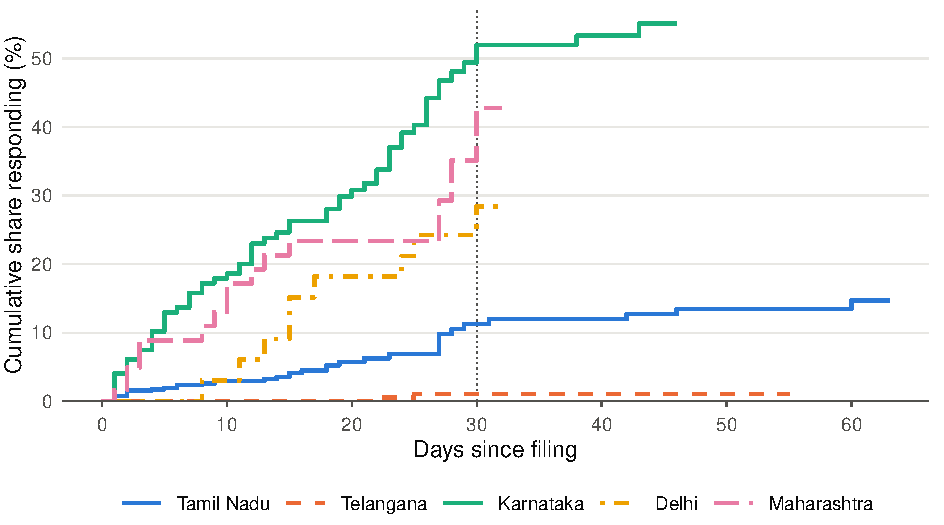
\includegraphics[width=\textwidth]{fig_km_state.pdf}
\begin{minipage}{\textwidth}\footnotesize
\textit{Notes:} Kaplan-Meier estimates of time to any response (any office action, including a transfer or fee demand), all 996 dated filings, censored at 29 October; curves stop when fewer than 10 applications remain at risk. Dotted line: the 30-day limit in s.7(1). Telangana is a lower bound because its portal sends no status emails.
\end{minipage}
\end{figure}

\FloatBarrier

\subsection{Effects of the legal reminder}
The estimated effect on any response within thirty days is \rtibtn{} percentage points in Tamil Nadu, with a standard error of \rtisetn{}, and \rtibother{} points in the other states, with a standard error of \rtiseother{}. Excluding Telangana from the latter group gives an estimate of \rtibextg{} points, with a standard error of \rtiseextg{}. These estimates leave considerable uncertainty about the size of the effect.

Table~\ref{tab:tab_main} reports results for all three outcomes. Estimates with additional department-group controls use fewer observations and rely on limited comparisons between letter versions within groups. Their larger coefficients should be assessed alongside that loss of information. The minimum-detectable-effect calculation in the table summarizes the precision of the current estimates; it is not a prospective power calculation. The evidence does not establish that reminders are ineffective, nor does it yet establish a reliable improvement in information provision.
\begin{table}[!htbp]
\centering
\caption{Effect of the legal-salience letter}
\label{tab:tab_main}
\small
\begin{adjustbox}{max width=\textwidth}
\begin{threeparttable}
\begin{tabular}{lrrrrrr}
\toprule
& \multicolumn{2}{c}{Tamil Nadu} & \multicolumn{2}{c}{Other states} & \multicolumn{2}{c}{Excl. Telangana} \\ \cmidrule(lr){2-3}\cmidrule(lr){4-5}\cmidrule(lr){6-7}  & (1) & (2) & (3) & (4) & (5) & (6) \\
\midrule
\addlinespace\multicolumn{7}{l}{\textit{Panel A. Any response by day 30}} \\
Legal letter & $-$0.1 & 1.1 & 3.6 & 7.4 & 10.9 & 32.8 \\
 & (6.0) & (5.8) & (3.9) & (3.8) & (9.3) & (13.4) \\
Plain-letter mean & 12.9 & 9.1 & 18.0 & 12.0 & 42.5 & 39.1 \\
Detectable effect (2.8 $\times$ SE) & 16.9 & 16.2 & 10.9 & 10.8 & 26.1 & 37.6 \\
Randomization-inference $p$ &  & 1.000 & 0.448 & 0.152 & 0.261 & 0.070 \\
N & 140 & 128 & 315 & 242 & 128 & 73 \\
\addlinespace\multicolumn{7}{l}{\textit{Panel B. Reply by day 30}} \\
Legal letter & 0.9 & 1.1 & 2.9 & 6.6 & 9.1 & 29.8 \\
 & (6.0) & (5.8) & (3.9) & (3.7) & (9.3) & (13.0) \\
Plain-letter mean & 11.8 & 9.1 & 16.6 & 11.4 & 39.1 & 37.0 \\
Detectable effect (2.8 $\times$ SE) & 16.7 & 16.2 & 10.8 & 10.3 & 26.0 & 36.4 \\
Randomization-inference $p$ &  & 1.000 & 0.550 & 0.172 & 0.322 & 0.126 \\
N & 140 & 128 & 315 & 242 & 128 & 73 \\
\addlinespace\multicolumn{7}{l}{\textit{Panel C. Information supplied by day 30}} \\
Legal letter & 2.1 & $-$1.1 & $-$2.4 & 1.0 & $-$3.6 & 7.9 \\
 & (4.2) & (3.5) & (3.3) & (2.6) & (8.0) & (9.5) \\
Plain-letter mean & 4.3 & 3.4 & 11.1 & 7.8 & 25.3 & 23.9 \\
Detectable effect (2.8 $\times$ SE) & 11.7 & 9.8 & 9.4 & 7.4 & 22.4 & 26.6 \\
Randomization-inference $p$ &  & 1.000 & 0.524 & 1.000 & 0.688 & 0.596 \\
N & 140 & 128 & 315 & 242 & 128 & 73 \\
\midrule
Randomization-block FE & No & Yes & Yes & Yes & Yes & Yes \\
Department-group FE & No & No & No & Yes & No & Yes \\
\bottomrule
\end{tabular}
\begin{tablenotes}[flushleft]\footnotesize
\item \textit{Notes:} Linear probability models, applications past day 30, percentage points, robust SEs. Legal letter: cites the s.7(1) deadline and s.20 penalties. Any response includes transfers and fee demands; reply excludes transfers; information: coded full or partial. Blocks: department $\times$ tier (Tamil Nadu), state $\times$ batch (others). Columns (4), (6) rest on 162, 41 applications in department groups with both letters.
\end{tablenotes}
\end{threeparttable}
\end{adjustbox}
\end{table}

\FloatBarrier

\section{Discussion}
The audit records a substantial difference between receiving an administrative response and obtaining requested information. This finding reinforces the distinction between response frequency and response quality in earlier RTI assessments and international audits \citep{raag2014,lagunes2019}. A system that counts transfers or disposal notices as completed cases can appear more responsive than one judged by the information an applicant receives. The present data document those stages separately, without assuming that an intermediate action constitutes refusal or final success.

The legal-reminder results remain uncertain. Earlier experiments show that explicit references to information law can improve responsiveness \citep{worthy2017,grimmelikhuijsen2019,spac2018}, but our comparison begins with applications already submitted through the statutory channel. A deadline-and-penalty reminder may offer a smaller additional signal. The present estimates cannot distinguish that possibility from limited precision, incomplete outcome observation, or differences in administrative capacity.

The results apply to one kind of request and to the offices reached so far. Information about an authority's own RTI administration is useful for comparing record access, but requests concerning benefits, personnel, procurement, or politically sensitive decisions may receive different treatment. Further follow-up will clarify how often transfers and fee demands lead to disclosure and how much missing portal and postal correspondence changes the recorded rates. Human validation of reply coding is also necessary to assess the accuracy of the content measures. These are the principal limits on interpreting the current evidence.

\bibliographystyle{apalike}
\bibliography{references}

\clearpage
\appendix
\section{Additional results}
Table~\ref{tab:tab_balance} reports filing and thirty-day follow-up by treatment arm among selected applications, and treatment composition by office level in Tamil Nadu. Table~\ref{tab:tab_content} describes the information contained in available replies. Table~\ref{tab:tab_robust} reports estimates with alternative controls and outcome windows. The samples change with the length of follow-up required, so differences across those specifications can reflect changes in sample composition as well as response timing.
\begin{table}[!htbp]
\centering
\caption{Does the letter predict who is filed and who has reached day 30?}
\label{tab:tab_balance}
\small
\begin{adjustbox}{max width=\textwidth}
\begin{threeparttable}
\begin{tabular}{lrrrrrrr}
\toprule
& & \multicolumn{3}{c}{Filed (\%)} & \multicolumn{3}{c}{Past day 30 (\%)} \\ \cmidrule(lr){3-5}\cmidrule(lr){6-8} State & N & Plain & Legal & $p$ & Plain & Legal & $p$ \\
\midrule
\addlinespace\multicolumn{8}{l}{\textit{Panel A. All drawn applications}} \\
Tamil Nadu & 1,000 & 52.0 & 53.7 & 0.867 & 13.3 & 15.7 & 0.901 \\
Telangana & 375 & 57.6 & 59.3 & 0.702 & 49.6 & 50.4 & 0.774 \\
Karnataka & 180 & 81.7 & 83.3 & 0.797 & 41.3 & 48.1 & 0.399 \\
Delhi & 44 & 100.0 & 100.0 &  & 50.0 & 50.0 &  \\
Maharashtra & 66 & 93.5 & 90.0 & 0.641 & 43.5 & 40.0 & 0.641 \\
\midrule
\addlinespace\multicolumn{8}{l}{\textit{Panel B. Tamil Nadu past day 30, by tier}} \\
 & N & Plain & Legal &  & Legal (\%) & Drawn (\%) &  \\
Department & 7 & 0 & 7 &  & 100.0 & 32.5 &  \\
Head of Department & 21 & 15 & 6 &  & 28.6 & 25.7 &  \\
Sub Office & 112 & 78 & 34 &  & 30.4 & 30.6 &  \\
\bottomrule
\end{tabular}
\begin{tablenotes}[flushleft]\footnotesize
\item \textit{Notes:} Past day 30: filed by 29 September. Panel A: $p$-values on the letter in a linear probability model with randomization-block fixed effects and robust SEs. Panel B: counts, with the legal share among them and among all drawn in that tier. All 7 department-tier filings past day 30 got the legal letter.
\end{tablenotes}
\end{threeparttable}
\end{adjustbox}
\end{table}

\FloatBarrier
\begin{table}[!htbp]
\centering
\caption{What the coded replies contain}
\label{tab:tab_content}
\small
\begin{adjustbox}{max width=\textwidth}
\begin{threeparttable}
\begin{tabular}{lrrrr}
\toprule
 & Tamil Nadu (26) & Others (78) & All (104) & All (\%) \\
\midrule
\addlinespace\multicolumn{5}{l}{\textit{Disposition}} \\
\quad Full information & 2 & 13 & 15 & 14 \\
\quad Partial information & 7 & 32 & 39 & 38 \\
\quad Fee asked first & 3 & 7 & 10 & 10 \\
\quad Denied or deflected & 9 & 6 & 15 & 14 \\
\quad Returned & 1 & 14 & 15 & 14 \\
\quad Transferred & 4 & 6 & 10 & 10 \\
\addlinespace\multicolumn{5}{l}{\textit{Data supplied}} \\
\quad Application-level register & 2 & 25 & 27 & 26 \\
\quad Monthly or category counts & 1 & 6 & 7 & 7 \\
\quad Period totals & 6 & 14 & 20 & 19 \\
\quad Prose only & 1 & 0 & 1 & 1 \\
\quad None & 16 & 33 & 49 & 47 \\
\addlinespace\multicolumn{5}{l}{\textit{Section 25 annual return}} \\
\quad Supplied & 3 & 19 & 22 & 21 \\
\quad Not held & 3 & 3 & 6 & 6 \\
\quad Offered on payment & 5 & 7 & 12 & 12 \\
\quad Told to apply separately & 0 & 2 & 2 & 2 \\
\quad Referred to website & 2 & 1 & 3 & 3 \\
\quad Not addressed & 13 & 46 & 59 & 57 \\
\addlinespace\multicolumn{5}{l}{\textit{How it arrived}} \\
\quad Post & 17 & 34 & 51 & 49 \\
\quad Portal & 7 & 26 & 33 & 32 \\
\quad Email & 2 & 18 & 20 & 19 \\
\addlinespace\multicolumn{5}{l}{\textit{Provisions cited}} \\
\quad Exemption, s.8 & 0 & 3 & 3 & 3 \\
\quad Sections 2(f) or 7(9) & 7 & 5 & 12 & 12 \\
\quad Transfer, s.6(3) & 0 & 6 & 6 & 6 \\
\quad None & 18 & 63 & 81 & 78 \\
\bottomrule
\end{tabular}
\begin{tablenotes}[flushleft]\footnotesize
\item \textit{Notes:} All 104 coded replies, whenever they came. Double-coded blind, with disagreements adjudicated. Fees were quoted in 16 replies (median Rs 37, maximum Rs 832).
\end{tablenotes}
\end{threeparttable}
\end{adjustbox}
\end{table}

\FloatBarrier
\begin{table}[!htbp]
\centering
\caption{Legal-salience letter: alternative specifications}
\label{tab:tab_robust}
\footnotesize
\begin{adjustbox}{max width=\textwidth}
\begin{threeparttable}
\begin{tabular}{lrrrrrr}
\toprule
& \multicolumn{2}{c}{Tamil Nadu} & \multicolumn{2}{c}{Other states} & \multicolumn{2}{c}{Excl. Telangana} \\ \cmidrule(lr){2-3}\cmidrule(lr){4-5}\cmidrule(lr){6-7}  & Coef. (SE) & N & Coef. (SE) & N & Coef. (SE) & N \\
\midrule
\addlinespace\multicolumn{7}{l}{\textit{Linear probability, any response (percentage points)}} \\
Baseline, by day 30 & 1.1 (5.8) & 128 & 3.6 (3.9) & 315 & 10.9 (9.3) & 128 \\
By day 35 & $-$0.1 (5.9) & 128 & 3.2 (3.7) & 269 & 13.3 (11.5) & 82 \\
By day 45 & 2.3 (5.6) & 128 & 3.5 (4.0) & 178 & 14.3 (16.5) & 40 \\
By day 14, all exposed that long & 0.0 (1.6) & 321 & 3.3 (3.4) & 392 & 6.4 (6.5) & 205 \\
Low-confidence matches as no response & 1.1 (5.8) & 128 & 4.0 (3.9) & 315 & 10.9 (9.3) & 128 \\
Adding RA fixed effects & 1.2 (5.8) & 128 & 3.7 (3.9) & 315 & 11.1 (9.4) & 128 \\
Adding filing-week fixed effects & 1.3 (5.8) & 128 & 4.0 (3.9) & 315 & 13.4 (9.3) & 128 \\
Excluding Maharashtra (shorter letter) &  &  & 3.5 (3.8) & 287 & 12.4 (10.4) & 100 \\
RA2 and RA4 filings only & 4.3 (8.6) & 57 & $-$1.2 (6.6) & 140 & $-$2.3 (12.4) & 77 \\
RA1 and RA3 filings only & 3.1 (8.0) & 65 & 6.4 (4.7) & 175 & 26.2 (14.6) & 51 \\
\addlinespace\multicolumn{7}{l}{\textit{Cox model, all filings (hazard ratio)}} \\
Legal letter, stratified by block & 1.16 (0.49) & 525 & 1.41 (0.31) & 471 & 1.46 (0.33) & 253 \\
\bottomrule
\end{tabular}
\begin{tablenotes}[flushleft]\footnotesize
\item \textit{Notes:} All rows: any response (any office action, including a transfer or fee demand), legal letter as in Table~\ref{tab:tab_main}, block fixed effects, robust SEs. Later cutoffs and the day-14 row use applications exposed that long. Filer-group rows are exploratory. The Cox model is our addition, not in the design document; its SE is on the hazard-ratio scale.
\end{tablenotes}
\end{threeparttable}
\end{adjustbox}
\end{table}

\FloatBarrier

\section{Analysis scope and data access}
This interim analysis emphasizes outcomes within thirty days, pools letter versions for the descriptive state comparisons, and adjusts for office-level composition only in Tamil Nadu. The broader study design envisages longer follow-up, descriptions based primarily on the plain letter, and additional analyses of appeals and the contents of RTI registers. Those analyses are not reported here. The survival regressions and permutation tests supplement the linear probability models. These interim results should be treated as exploratory.

The replication materials contain de-identified analytical data, application assignments, coding decisions, and code for the reported results. Original emails and documents contain personal information and are held separately. Details of data construction, the analysis plan, and the computational environment are documented with the replication materials.
\end{document}
